%; whizzy paragraph -pdf xpdf -latex ./whizzypdfptex.sh
%; whizzy-paragraph "^\\\\begin{frame}\\|\\\\emtext"
% latex beamer presentation.
% platex, latex-beamer $B$G%3%s%Q%$%k$9$k$3$H$rA[Dj!#(B 

%     Tokyo Debian Meeting resources
%     Copyright (C) 2012 Junichi Uekawa

%     This program is free software; you can redistribute it and/or modify
%     it under the terms of the GNU General Public License as published by
%     the Free Software Foundation; either version 2 of the License, or
%     (at your option) any later version.

%     This program is distributed in the hope that it will be useful,
%     but WITHOUT ANY WARRANTY; without even the implied warreanty of
%     MERCHANTABILITY or FITNESS FOR A PARTICULAR PURPOSE.  See the
%     GNU General Public License for more details.

%     You should have received a copy of the GNU General Public License
%     along with this program; if not, write to the Free Software
%     Foundation, Inc., 51 Franklin St, Fifth Floor, Boston, MA  02110-1301 USA

\documentclass[cjk,dvipdfmx,12pt]{beamer}
\usetheme{Tokyo}
\usepackage{monthlypresentation}

%  preview (shell-command (concat "evince " (replace-regexp-in-string "tex$" "pdf"(buffer-file-name)) "&")) 
%  presentation (shell-command (concat "xpdf -fullscreen " (replace-regexp-in-string "tex$" "pdf"(buffer-file-name)) "&"))
%  presentation (shell-command (concat "evince " (replace-regexp-in-string "tex$" "pdf"(buffer-file-name)) "&"))

%http://www.naney.org/diki/dk/hyperref.html
%$BF|K\8l(BEUC$B7O4D6-$N;~(B
\AtBeginDvi{\special{pdf:tounicode EUC-UCS2}}
%$B%7%U%H(BJIS$B7O4D6-$N;~(B
%\AtBeginDvi{\special{pdf:tounicode 90ms-RKSJ-UCS2}}

\newenvironment{commandlinesmall}%
{\VerbatimEnvironment
  \begin{Sbox}\begin{minipage}{1.0\hsize}\begin{fontsize}{8}{8} \begin{BVerbatim}}%
{\end{BVerbatim}\end{fontsize}\end{minipage}\end{Sbox}
  \setlength{\fboxsep}{8pt}
% start on a new paragraph

\vspace{6pt}% skip before
\fcolorbox{dancerdarkblue}{dancerlightblue}{\TheSbox}

\vspace{6pt}% skip after
}
%end of commandlinesmall

\title{$BEl5~%(%j%"(BDebian$BJY6/2q(B}
\subtitle{$BBh(B102$B2s(B 2013$BG/(B7$B7nEY(B}
\author{$B>e@n=c0l(B}
\date{2013$BG/(B7$B7n(B20$BF|(B}
\logo{
\includegraphics[width=8cm]{image200607/openlogo-light.eps}}

\begin{document}

\begin{frame}
\titlepage{}
\end{frame}

\begin{frame}{$B@_1D=`Hw$K$46(NO$/$@$5$$!#(B}
$B2q>l@_1D$h$m$7$/$*$M$,$$$7$^$9!#(B
\end{frame}

\begin{frame}{Agenda}
\begin{minipage}[t]{0.45\hsize}
  \begin{itemize}
  \item $BCm0U;v9`(B
	\begin{itemize}
	 \item $B0{?)6X;_(B
	\end{itemize}
   \item $B:G6a$"$C$?(BDebian$B4XO"$N%$%Y%s%HJs9p(B
	\begin{itemize}
        \item $BBh(B100$B2s(B $BEl5~%(%j%"(BDebian$BJY6/2q(B
        \item 2013 $BBgE}0l(BDebian$BJY6/2q(B
	\end{itemize}
 \end{itemize}
\end{minipage} 
\begin{minipage}[t]{0.45\hsize}
 \begin{itemize}
  \item Debian Trivia Quiz
  \item $B;vA02]Bj>R2p(B
 \end{itemize}
\end{minipage}
\end{frame}

\section{$B%$%Y%s%HJs9p(B}
\emtext{$B%$%Y%s%HJs9p(B}

\begin{frame}{$BBh(B100$B2s(B $BEl5~%(%j%"(BDebian$BJY6/2q(B}
 $B!!(B
\end{frame}

\begin{frame}{$BBgE}0l(BDebian$BJY6/2q(B 2013}
\end{frame}

\section{DWN quiz}
\emtext{DWN quiz}
\begin{frame}{Debian $B>o<1%/%$%:(B}

  Debian $B$N>o<1!"$b$A$m$sCN$C$F$^$9$h$M(B?
$BCN$i$J$$$J$s$FCQ$:$+$7$/$F!"CN$i$J$$$H$O8@$($J$$$"$s$J$3$H$d$3$s$J$3$H!"(B
$B$_$s$J$G3NG'$7$F$_$^$7$g$&!#(B

$B:#2s$N=PBjHO0O$O(B\url{debian-devel-announce@lists.debian.org},
\url{debian-devel@lists.debian.org} $B$KEj9F$5$l$?(B
$BFbMF$H(BDebian Project News$B$J$I$+$i$G$9!#(B

\end{frame}

\subsection{$BLdBj(B}
%; whizzy-master ../debianmeetingresume201211.tex
% 以上の設定をしているため、このファイルで M-x whizzytex すると、whizzytexが利用できます。
%

\santaku
{Stefano Zacchiroli さんが新しく作成したサービスは?}
{chiebukuro.debian.net}
{2ch.debian.net}
{sources.debian.net}
{C}
{Stefano Zacchiroli さんが、Debian パッケージで提供されているソースコードすべてを閲覧・検索出来るsources.debian.netを作った}

\santaku
{新しく FTP master チームに入った人は?}
{Gergely Nagy} % 2012 DPL立候補者 % dh-exec 開発者
{Kouhei Maeda}
{Joerg Jaspert}
{A}
{Paul Tagliamonte,Scott Kitterman,Luke Faraone, Gergely Nagy が加入}

\santaku
{Debian GNU/Hurd がリリースされましたが、バージョンはいくつでしょう。}
{2013}
{3.141592}
{7.0}
{A}
{}



\section{$B;vA02]Bj(B}
\emtext{$B;vA02]Bj(B}
{\footnotesize
% 
\begin{prework}{ koedoyoshida }

\begin{enumerate}
\item お使いのマシンにARMはありますか?もしあるのでしたら、どのように使っ
ているか教えてください。\\
Raspberry Piを使ってます。
とりあえずリモートアクセス用がメインですが、
I2Cとかを使って外部IOをやってみたいと思っています。
\item  Debian のARM に期待していること、お願いしたいことがあれば教えてくだ
さい。\\
省電力な環境を生かしてReadOnlyboot(でも定期的にセキュリティupdateはし
たい)で放置できる環境とかが作れるとよいですね。
\end{enumerate}

\end{prework}

\begin{prework}{ 吉野 }
\begin{enumerate}
\item  地図マシンです
\item なし 
\end{enumerate}
\end{prework}

\begin{prework}{ dictoss}
\begin{enumerate}
\item  CuBoxを持っている。eSATA端子があるのでファイルサーバのバックアップ
をするマシンとして使おうとしたが、USBポートから電源供給量が不足のため、
HDDが動かず使えていない。そのため単なるarmelバイナリのお試しマシンになっ
ている。

\item  新Nexus7でDebianが動いてほしい。
\end{enumerate}
\end{prework}

\begin{prework}{ mtoshi.g }
\begin{enumerate}
\item  お使いのマシンにARMはありますか?\\
ないっす

\item  Debian のARM に期待していること、お願いしたいことがあれば教えてくだ
さい。\\
今のところないっす
\end{enumerate}
\end{prework}

\begin{prework}{ 野島 貴英 }
\begin{enumerate}
\item  昔売っていたB\&NのNookColorをARM機材実験ボードとして未だに使ってます。
この電子書籍端末は2012/4の東京エリアdebian勉強会,2012/6の大統一debian
勉強会で喋ったとおり、特定ブートフォーマットのSDカードを用意してSDカー
ドスロットへ入れちゃうと、うっかりそのままブートしちゃうという隠れ(?)
機能が大変便利です。おまけに連続8回起動失敗するとリカバリーが始まると
いう非文鎮化機能まで搭載しています。そのままでもpdfリーダ、ポータブル
mp4ビデオ/mp3鑑賞機材として、また、debian ARMのnativeブートの可能性を
秘めたhack機材としても楽しくお使いいただけます。
\item  NookColor用のdebianネイティブブートが可能なイメージ(というかインス
  トーラ)が欲しいといってみるテスト。
\end{enumerate}
\end{prework}

\begin{prework}{ 岩松 信洋 }
\begin{enumerate}
\item  お使いのマシンにARMはありますか?もしあるのでしたら、どのように使っ
ているか教えてください。\\
たくさんある。開発用とかビルドマシンとして使っています。
Raspberry Pi は家のゲートウェイマシンとして動いています。
\item  Debian のARM に期待していること、お願いしたいことがあれば教えてくだ
さい。\\
マルチメディア系が弱いので整備して欲しい。
\end{enumerate}

\end{prework}

\begin{prework}{ 上川純一 }
なし
\end{prework}

\begin{prework}{ まえだこうへい }
\begin{enumerate}
\item  Armadillo Jで自宅内のDHCPサーバとして使っています(not Debian)。
OpenBlockS AX3を、昨年夏ごろにカッとなって作ったioriというツール(最近
話題のdockerみたいなの)の開発環境として使っています。
\item  今は特にないですが、今後ARMサーバの製品版が出てきた時にd-iでインス
トールできることでしょうか。
\end{enumerate}
\end{prework}

}

\section{armmp}
\emtext{armmp}

\section{$B7n4)(BDebhelper}
\emtext{$B7n4)(BDebhelper}
\begin{frame}{$B:#7n$N%3%^%s%I(B}
\begin{center}
\Huge
 dh\_strip
\end{center}
\end{frame}

\begin{frame}{dh\_strip$B$N5!G=(B}

\begin{itemize}
\item $B<B9T%P%$%J%j!"6&M-%i%$%V%i%j!"@EE*%i%$%V%i%j$+$i!"%G%P%C%0%7%s%\%k$r<h$j=|$/!#(B
\item $B<h$j=|$$$?%G%P%C%0%7%s%\%k$r%G%P%C%,$,8+$D$1$l$k$h$&$K$7$F!"(B*-dbg$B%Q%C%1!<%8$,:n$j$d$9$$$h$&$K%S%k%I%G%#%l%/%H%j0J2<$KG[CV$9$k(B
\end{itemize}

\end{frame}

\begin{frame}{$B$I$&$d$C$F(B*-dbg$B%Q%C%1!<%8$r:n$k!)(B}

$B!!$=$s$J$"$J$?$K!"(B\\
\begin{center}
\LARGE
2012$BG/(B $BBgE}0l(BDebian$BJY6/2q(B\\
$B!V(Bdebug.debian.net$B!W$N(B\\
$B%W%l%<%s;qNA$,$*$9$9$a!*(B
\end{center}
\begin{center}
\url{http://gum.debian.or.jp/2012/}
\end{center}

$B!!$H$j$"$($:!"$9$G$KH/I=:Q$_$J$N$G!"$3$3$G$O>JN,!#(B

\end{frame}

\begin{frame}{dh\_strip$B$N%3%^%s%I%i%$%s%*%W%7%g%s(B($B$=$N(B1)}

\begin{itemize}
\item man debhelper$B$K5-:\$5$l$F$$$k(Bdebhelper$B6&DL%*%W%7%g%s(B\\
$B!!B>$N7n4)(Bdebhelper$B$NH/I=$G$J$5$l$F$$$k$H$*$j$J$N$G!"$3$3$G$O3d0&!#(B
\item -Xitem,--exclude=item \\
  item$B$H$$$&L>A0$r;}$D%U%!%$%kL>$KBP$7$F$O=hM}$r9T$$$^$;$s!#J#?t;XDj$7$?$1$l$P!"(B
``dh\_strip -Xfoo1 -Xfoo2''$B$HJ#?t$J$i$Y$F;XDj$,$G$-$^$9!#(B
\item --dbg-package=package \\
*-dbg$B%Q%C%1!<%8$r:n$k:]$K!"%G%P%C%0%7%s%\%k$r3JG<$9$k%Q%C%1!<%8L>$r;XDj$9$k0Y$KMxMQ$7$^$9!#(Bdebhelper$B$N(BCOMPATIBILITY LEVEL$B$K$h$C$F?6$kIq$$$,JQ$o$j$^$9!#(B($B8e=R(B)
\end{itemize}

\end{frame}

\begin{frame}{dh\_strip$B$N%3%^%s%I%i%$%s%*%W%7%g%s(B($B$=$N(B2)}
\begin{itemize}
\item -k \\
$B%G%P%C%0%7%s%\%k$r%P%$%J%j%Q%C%1!<%8$K4^$a$F$7$^$$$^$9!#$D$^$j!"%P%$%J%j$,%$%s%9%H!<%k$5$l$k$HF1;~$K!"BP1~$7$?%G%P%C%0%7%s%\%k$b(B/usr/lib/debug/$B0J2<$K%$%s%9%H!<%k$5$l$k$h$&$J%Q%C%1!<%8$r:n@.$9$k$H$-$K;H$$$^$9!#$J$*!"(B--dbg-package$B$b;XDj$5$l$k$H!"(B--dbg-package$B$NJ}$NF0:n$,M%@h$5$l$^$9!#(B
\end{itemize}

\end{frame}

\begin{frame}{dh\_strip$B$N(BCOMPATIBILITY LEVEL$B$NF0:n$N0c$$(B($B$=$N(B1)}

$B0J2<$O(B--dbg-package$B;XDj;~$N(Bdh\_strip$B$N?6$kIq$$$N0c$$!#(B

\begin{itemize}
\item 4$B0J2<(B\\
$B!!(B``dh\_strip --dbg-package=xxxx --dbg-package=yyyy''$B$N$h$&$K(B--dbg-package
$B$rJ#?t;XDj$9$k;v$,=PMh$^$9!#$3$3$G!"$3$A$i$G;XDj$7$?L>A0(B(xxxx$B$d!"(Byyyy)$B$K9gCW$9$k(B
$B%Q%C%1!<%8$r=hM}$9$k:]!"(B''$B%Q%C%1!<%8L>(B-dbg''$B$H$$$&%Q%C%1!<%8L>$r(B*-dbg$B%Q%C%1!<%8(B
$B$N%Q%C%1!<%8L>$H$7$F<+F0E*$KMxMQ$7$^$9!#$^$?!"$3$N(BCOMPATIBILITY LEVEL$B$N>l9g!"(B
$B%=!<%9%Q%C%1!<%8$K4^$^$l$k(Bdebian/control$B$K$O!"$3$l$i(B*-dbg$B%Q%C%1!<%8$N0Y$N(B
$B5-=R$rI,MW$H$O$7$F$$$^$;$s!#(B
\end{itemize}

\end{frame}

\begin{frame}{dh\_strip$B$N(BCOMPATIBILITY LEVEL$B$NF0:n$N0c$$(B($B$=$N(B2)}

\begin{itemize}
\item 5$B0J>e(B\\
--dbg-package$B$O#1$D;XDj$9$k$N$,86B'$H$J$j$^$9!#$b$7J#?t;XDj$7$?>l9g$O!"(B
$B:G=i$K;XDj$5$l$?FbMF$N$_MxMQ$5$l$^$9!#$^$?!"(B--dbg-package=xxxxx$B$H$9$k$H!"%G%P%C(B
$B%0%7%s%\%k$r3JG<$9$k%Q%C%1!<%8L>$H$7$F!"(Bxxxxx$B$,$=$N$^$^;H$o$l$^$9!#Nc$($P!"(Blibfo
o$B%Q%C%1!<%8$H!"(Bfoo$B%Q%C%1!<%8$r9=C[$7!"$3$l$i%Q%C%1!<%8$K4^$^$l$F$$$k%P%$%J%j$N%G(B
$B%P%C%0%7%s%\%k$r(Bfoo-dbg$B%Q%C%1!<%8$KA4ItF~$l$k$K$O!"(B--dbg-package=foo-dbg$B$H;XDj$7(B
$B$^$9!#$^$?!"%=!<%9%Q%C%1!<%8$K4^$^$l$k(Bdebian/control$B$K$O!"(B
$B@8@.M=Dj$N(B*-dbg$B%Q%C%1!<%8$N0Y$N5-=R$OI,?\$H$J$j!"K|0l5-:\$5$l$F$$$J$$>l9g$O(B
$B%(%i!<$H$7$F07$o$l!"$3$N>l9g$O(Bdh\_strip$B$O%(%i!<$rI=<($7$F=*N;$7$^$9!#(B
\end{itemize}

\end{frame}

\begin{frame}{dh\_strip$B$N(BCOMPATIBILITY LEVEL$B$NF0:n$N0c$$(B($B$=$N(B3)}

$B0J2<$O(B-k/--dbg-package$B;XDj;~$N=PMh>e$,$k%G%P%C%0%7%s%\%k%U%!%$%k$N0c$$(B

\begin{itemize}
\item 8$B0J2<(B\\
 ``/usr/lib/debug/+$B%P%$%J%j$N%$%s%9%H!<%k@h%Q%9(B/+$B%P%$%J%j%U%!%$%kL>(B''$B$K3J(B
$BG<$5$l$k$h$&$K%G%P%C%0%7%s%\%k%U%!%$%k$,@8@.$5$l$^$9!#$^$?!"%G%P%C%0$K4X$9$k>pJs(B
$B$O%3%s%Q%$%i$,@8@.$7$?$^$^$N7A$GJ]B8$5$l$k$?$a!"%G%P%C%0%7%s%\%k%U%!%$%k$N%5%$%:(B
$B$OBg$-$/$J$j$,$A$G$9!#(B
\end{itemize}

\end{frame}

\begin{frame}{dh\_strip$B$N(BCOMPATIBILITY LEVEL$B$NF0:n$N0c$$(B($B$=$N(B4)}
\begin{itemize}
\item 9$B0J>e(B\\
$B%P%$%J%j$,(BBuildID$B$r4^$s$G$$$k>l9g$O!"(B
``/usr/lib/debug/.build-id/BuildID$B$N>e0L(B2$B7e(B/+BuildID$B$N;D$j$N7e(B+.debug''
$B$K3JG<$5$l$k$h$&$K%G%P%C%0%7%s%\%k%U%!%$%k$,@8@.$5$l$^$9!#(BBuildID$B$r4^$s$G(B
$B$$$J$1$l$P(BCOMPATIBILITY LEVEL 8$B0J2<$HF1MM$N%U%!%$%kL>$H$J$j$^$9!#(B
$B$^$?!"(BBuildID$B$NM-L5$K$+$+$o$i$:!"%G%P%C%0$K4X$9$k>pJs$O(Bzlib$B$K$h$j(B
$B05=L$5$l$F3JG<$5$l$^$9!#$=$N$?$a!"%G%P%C%0%7%s%\%k%U%!%$%k$N%5%$%:$O$G$-$k$@$1(B
$B>.$5$/$J$k$h$&$K$J$C$F$$$^$9!#(B
\end{itemize}

\end{frame}

\begin{frame}[containsverbatim]{$B$H$3$m$G(BBuildID$B$C$F(B}

 file$B%3%^%s%I$G%P%$%J%j$rD4$Y$k$H=P$F$-$^$9!#(B

\begin{commandline}
$ file /usr/bin/gst-launch
/usr/bin/gst-launch: ELF 64-bit LSB  executable, 
x86-64, version 1 (SYSV), dynamically linked 
(uses shared libs), for GNU/Linux 2.6.26, 
BuildID[sha1]=9b42db476118ab2b81041acd80e45e89e4289ea2, 
stripped
\end{commandline}
%$
 
 $B>\$7$/$O(B2013$BG/BgE}0l(BDebian$BJY6/2q!V(Bgdb+python$B3HD%$r;H$C$?%G%P%C%0<jK!!W(B
(\url{http://gum.debian.or.jp/2013/slide_data_list})$B$K5-:\$7$F$^$9!#(B

\end{frame}

\begin{frame}{$B%G%P%C%0%7%s%\%k%U%!%$%k$N7A<0(B}

 Debian$B$N(Bi386/amd64$BMQ(Blinux$B%7%9%F%`$G$O!"%G%P%C%0%7%s%\%k%U%!%$%k$N7A<0$H$7$F(B
$B$[$\(BDWARF$B$J%G%P%C%0%7%s%\%k%U%!%$%k$,MxMQ$5$l$F$$$^$9!#(BDWARF$B$O(B
$B<B9T%U%!%$%k$N7A<0$G$"$k(BELF$B%U%)!<%^%C%H$r%Y!<%9$K:n$i$l$F$$$k$?$a!"(B
DWARF$B$rM}2r$9$k;~$K$O!"(BELF$B$b$"$o$;$FCN$C$F$*$/$HNI$$$G$9!#(B

\end{frame}

\begin{frame}{DWARF$BJ88%(B}
$B!!(BDWARF$B$K$D$$$F!'(B\\
\begin{itemize}
\item $BK\2H(B \\
\url{http://www.dwarfstd.org/}
\item $B7k9=NI$$2r@b5-;v(B \\
\url{http://www.ibm.com/developerworks/jp/opensource/library/os-debugging/}\\
\url{http://ja.wikipedia.org/wiki/DWARF}\\
\item DWARF$B$rM}2r$9$k0Y$N$*6!$K(BELF$B$b$I$&$>!*(B\\
\url{http://ja.wikipedia.org/wiki/Executable_and_Linkable_Format}
\end{itemize}
\end{frame}


\begin{frame}[containsverbatim]{$B%G%P%C%0%7%s%\%k%U%!%$%kGA$$$F$_$k(B}

$B$^$:!"PmbW$7$F$_$?$$$N$G!"3F%X%C%@!"3F%;%/%7%g%s$rPmbW$7$F$_$^$9!#(B
\begin{commandlinesmall}
$ sudo aptitude install binutils/sid php5-dbg
$ env LANG=C readelf -e /usr/lib/debug/usr/bin/php5
ELF Header:
  Magic:   7f 45 4c 46 02 01 01 00 00 00 00 00 00 00 00 00 
  Class:                             ELF64
..$BCfN,(B...
  Start of program headers:          64 (bytes into file)
  Start of section headers:          19669080 (bytes into file)
...$BCfN,(B...
Section Headers:
  [Nr] Name              Type             Address           Offset
       Size              EntSize          Flags  Link  Info  Align
...$BCfN,(B...
  [ 1] .interp           NOBITS           0000000000400238  00000238
       000000000000001c  0000000000000000   A       0     0     1
...$BCfN,(B...
  [28] .debug_aranges    PROGBITS         0000000000000000  000002d0
       0000000000006190  0000000000000000           0     0     1
...$BCfN,(B...  
\end{commandlinesmall} 
$B$3$3$G$O;fLL$,$;$^$$$N$G!"3'$5$s$*<j85$N(Bdebian$B%^%7%s$G(B
$B3NG'$7$F$_$F$/$@$5$$$^$;!#(B
\end{frame}

\begin{frame}{readelf -e $B$N7k2L$r?^<($7$F$_$k(B}

\begin{center}
\includegraphics[height=0.70\textheight]{image201307/dwarf-top-headers.eps}
\end{center}

\end{frame}

\begin{frame}[containsverbatim]{$B%=!<%9$N>pJs$r8+$F$_$k(B($B$=$N(B1)}
 .debug\_info$B%;%/%7%g%s$K(BDWARF$B$N$H$*$j$K3JG<$5$l$F$$$k!#$G!"(B
$B$3$A$i$N%G%3!<%I$K$O(Breadelf -wi$B$,JXMx!#(B
\begin{commandlinesmall}
$  env LANG=C readelf -wi /usr/lib/debug/usr/bin/php5
Contents of the .debug_info section:

  Compilation Unit @ offset 0x0:
   Length:        0x15bf3 (32-bit)
   Version:       4
   Abbrev Offset: 0x0
   Pointer Size:  8
 <0><b>: Abbrev Number: 1 (DW_TAG_compile_unit)
    <c>   DW_AT_producer    : (indirect string, offset: 0x1832): 
           GNU C 4.8.1 -mtune=generic 
           -march=x86-64 -g -O2 -fstack-protector -fPIC 
           --param ssp-buffer-size=4  
    <10>   DW_AT_language    : 1        (ANSI C)
    <11>   DW_AT_name        : 
    (indirect string, offset: 0x1955): /tmp/buildd/php5-5.5.0+dfsg/ext/date/
     php_date.c   
    <15>   DW_AT_comp_dir    : (indirect string, offset: 0x6f0): 
      /tmp/buildd/php5-5.5.0+dfsg/cli-build 
\end{commandlinesmall}
%$
\end{frame}

\begin{frame}[containsverbatim]{$B%=!<%9$N>pJs$r8+$F$_$k(B($B$=$N(B2)}

 readelf -wi$B$N7k2L$+$i!"$3$A$i$N(BCompilation Unit($B0J2<(BCU)$B$K5-:\$5$l$F$$$k%=!<%9%U%!%$%k(B($B0J2<(BDW\_AT\_name)$B$O!"(B
/tmp/buildd/php5-5.5.0+dfsg/ext/date/php\_date.c$B$G$"$j!"(B
$B%3%s%Q%$%k$,9T$o$l$?%G%#%l%/%H%j(B($B0J2<(BDW\_AT\_comp\_dir)$B$O(B
/tmp/buildd/php5-5.5.0+dfsg/cli-build$B$H$J$j$^$9!#(B

\end{frame}

\begin{frame}{Use the SOURCE!($B$=$N(B1)}
$B!!(B.debug\_info$B$N(BCU$B$N(BDW\_AT\_name$B$,@dBP%Q%9$G5-:\$5$l$F$$$k$h$&$J>l9g$O!"(B
gdb$B$G!"(Bset substitute-path$B$K(BDW\_AT\_name$B$N@dBP%Q%9ItJ,$r;XDj$7$^$9(B
$B6qBNNc"-(B
\begin{center}
\LARGE
2013$BG/(B $BBgE}0l(BDebian$BJY6/2q(B\\
$B!V(Bgdb+python$B3HD%$r;H$C$?%G%P%C%0<jK!!W(B
$B$N%W%l%<%s;qNA(B
\end{center}
\begin{center}
\url{http://gum.debian.or.jp/2013/slide_data_list}
\end{center}

\end{frame}

\begin{frame}[containsverbatim]{Use the SOURCE!($B$=$N(B2)}
$B!!(B.debug\_info$B$N(BCU$B$N(BCU$B$N(BDW\_AT\_name$B$,AjBP%Q%9(B($B$"$k$$$O!"%U%!%$%kL>$=$N$b$N!K$G5-:\$5$l$F$$$k$h$&$J>l9g$O!"(Bgdb$B$G!"(Bset substitute-path$B$K$O(BDW\_AT\_comp\_dir$B$N@dBP%Q%9ItJ,$r;XDj$7$^$9!#(B
$B6qBNNc"-(B
\begin{commandlinesmall}
$ env LANG=C readelf -wi /usr/lib/debug/.build-id/9b/42db476118ab2b81041acd80e45e89e4289ea2.debug
...$BCfN,(B...
    <11>   DW_AT_name        : (indirect string, offset: 0x57a): gst-run.c      
    <15>   DW_AT_comp_dir    : (indirect string, offset: 0x36b): 
          /tmp/buildd/gstreamer0.10-0.10.36/tools        
...$BCfN,(B...
$ gdb --args gst-launch
(gdb) set substitute-path /tmp/buildd/ /home/yours/debian-src/gstreamer/
(gdb) b main
(gdb) run
(gdb) l
313       return candidates;
314     }
315     
316     int
317     main (int argc, char **argv)
319       GHashTable *candidates;
320       gchar *dir;
\end{commandlinesmall}
\end{frame}

\begin{frame}{Use the SOURCE!($B$=$N(B3)}
 gdb$B$O!"%=!<%9$N0LCV$r5a$a$k$H$-$K0J2<$N%"%k%4%j%:%`$K=>$C$F%=!<%9$N0LCV$r5a$a$h$&$H$7$^$9!#(B

$B!!(B\begin{itemize}
   \item CU$B$K5-:\$5$l$F$$$k%U%!%$%kL>$,@dBP%Q%9$N;~(B:\\
 $B$=$N$^$^%=!<%9%U%!%$%k$N0LCV$H$7$F07$&!#$^$?!"$3$N;~(BDW\_AT\_comp\_dir$B$N>pJs$OL5;k$5$l$k!#(B
  \item CU$B$K5-:\$5$l$F$$$k%U%!%$%kL>$,AjBP%Q%9$N;~(B:\\
 $B%=!<%9$N%U%!%$%kL>$r(B''DW\_AT\_comp\_dir$B$NCM(B''+''/''+''DW\_AT\_name''$B$H$7$F07$&!#(B
$B!!(B\end{itemize}

$B$J$N$G!"@h$[$I$NDL$j(Bset substitute-path$B$N85%G%#%l%/%H%j>pJs$H$7$F;XDj$9$k%Q%9>pJs$,0[$J$j$^$9!#(B

\end{frame}

\begin{frame}[containsverbatim]{$B;29M!'(BCOMPATIBILITY LEVEL9$B$@$H(B...($B$=$N(B1)}
$B%G%P%C%0%7%s%\%k$,(BCOMPATIBILITY LEVEL9$B$N85$G:n@.$5$l$F$$$k$H(B...
\begin{commandlinesmall}
$ sudo aptitude install libgstreamer0.10-0-dbg
$ env LANG=C readelf -e /usr/lib/debug/.build-id/9b/42db476118ab2b81041
acd80e45e89e4289ea2.debug
...$BCfN,(B...
  [28] .zdebug_aranges   PROGBITS         0000000000000000  000002d0
       000000000000002f  0000000000000000           0     0     1
  [29] .zdebug_info      PROGBITS         0000000000000000  000002ff
       0000000000000ccd  0000000000000000           0     0     1
...$BCfN,(B...
\end{commandlinesmall}
$BA4It!"(B''.z+debug+$B$J$s$H$+(B''$B$K%;%/%7%g%sL>$,JQ99$5$l$F$$$^$9!#(B
\end{frame}

\begin{frame}[containsverbatim]{$B;29M!'(BCOMPATIBILITY LEVEL9$B$@$H(B...($B$=$N(B2)}
 .zdebug\_info$B%;%/%7%g%s$r%@%s%W$7$F$_$?!#(B
\begin{commandlinesmall}
$ env LANG=C readelf -x .zdebug_info /usr/lib/debug/.build-id/9b/42
db476118ab2b81041acd80e45e89e4289ea2.debug
Hex dump of section '.zdebug_info':
  0x00000000 5a4c4942 00000000 00001b3f 789c7d59 ZLIB.......?x.}Y
  0x00000010 7b7454c5 199fefee 6e76b3d9 2497cd7b {tT.....nv..$..{
  0x00000020 370b2109 012e0482 243c13d8 84f01079 7.!.....$<.....y
  0x00000030 05437988 0887444f 44501e25 94a788b6 .Cy...DODP.%....
\end{commandlinesmall}
%$
$B$H$$$&$o$1$G!"(BZLIB$B$G05=L$5$l$F$^$9!#(B
\end{frame}

\begin{frame}{$B$*$o$j$K(B}
\begin{center}
\Huge
 $B<ALd$J$I$*$M$,$$$7$^$9!<(B
\end{center}
\end{frame}

\section{raspberry pi}
\emtext{raspberry pi}

\begin{frame}{raspberry pi}
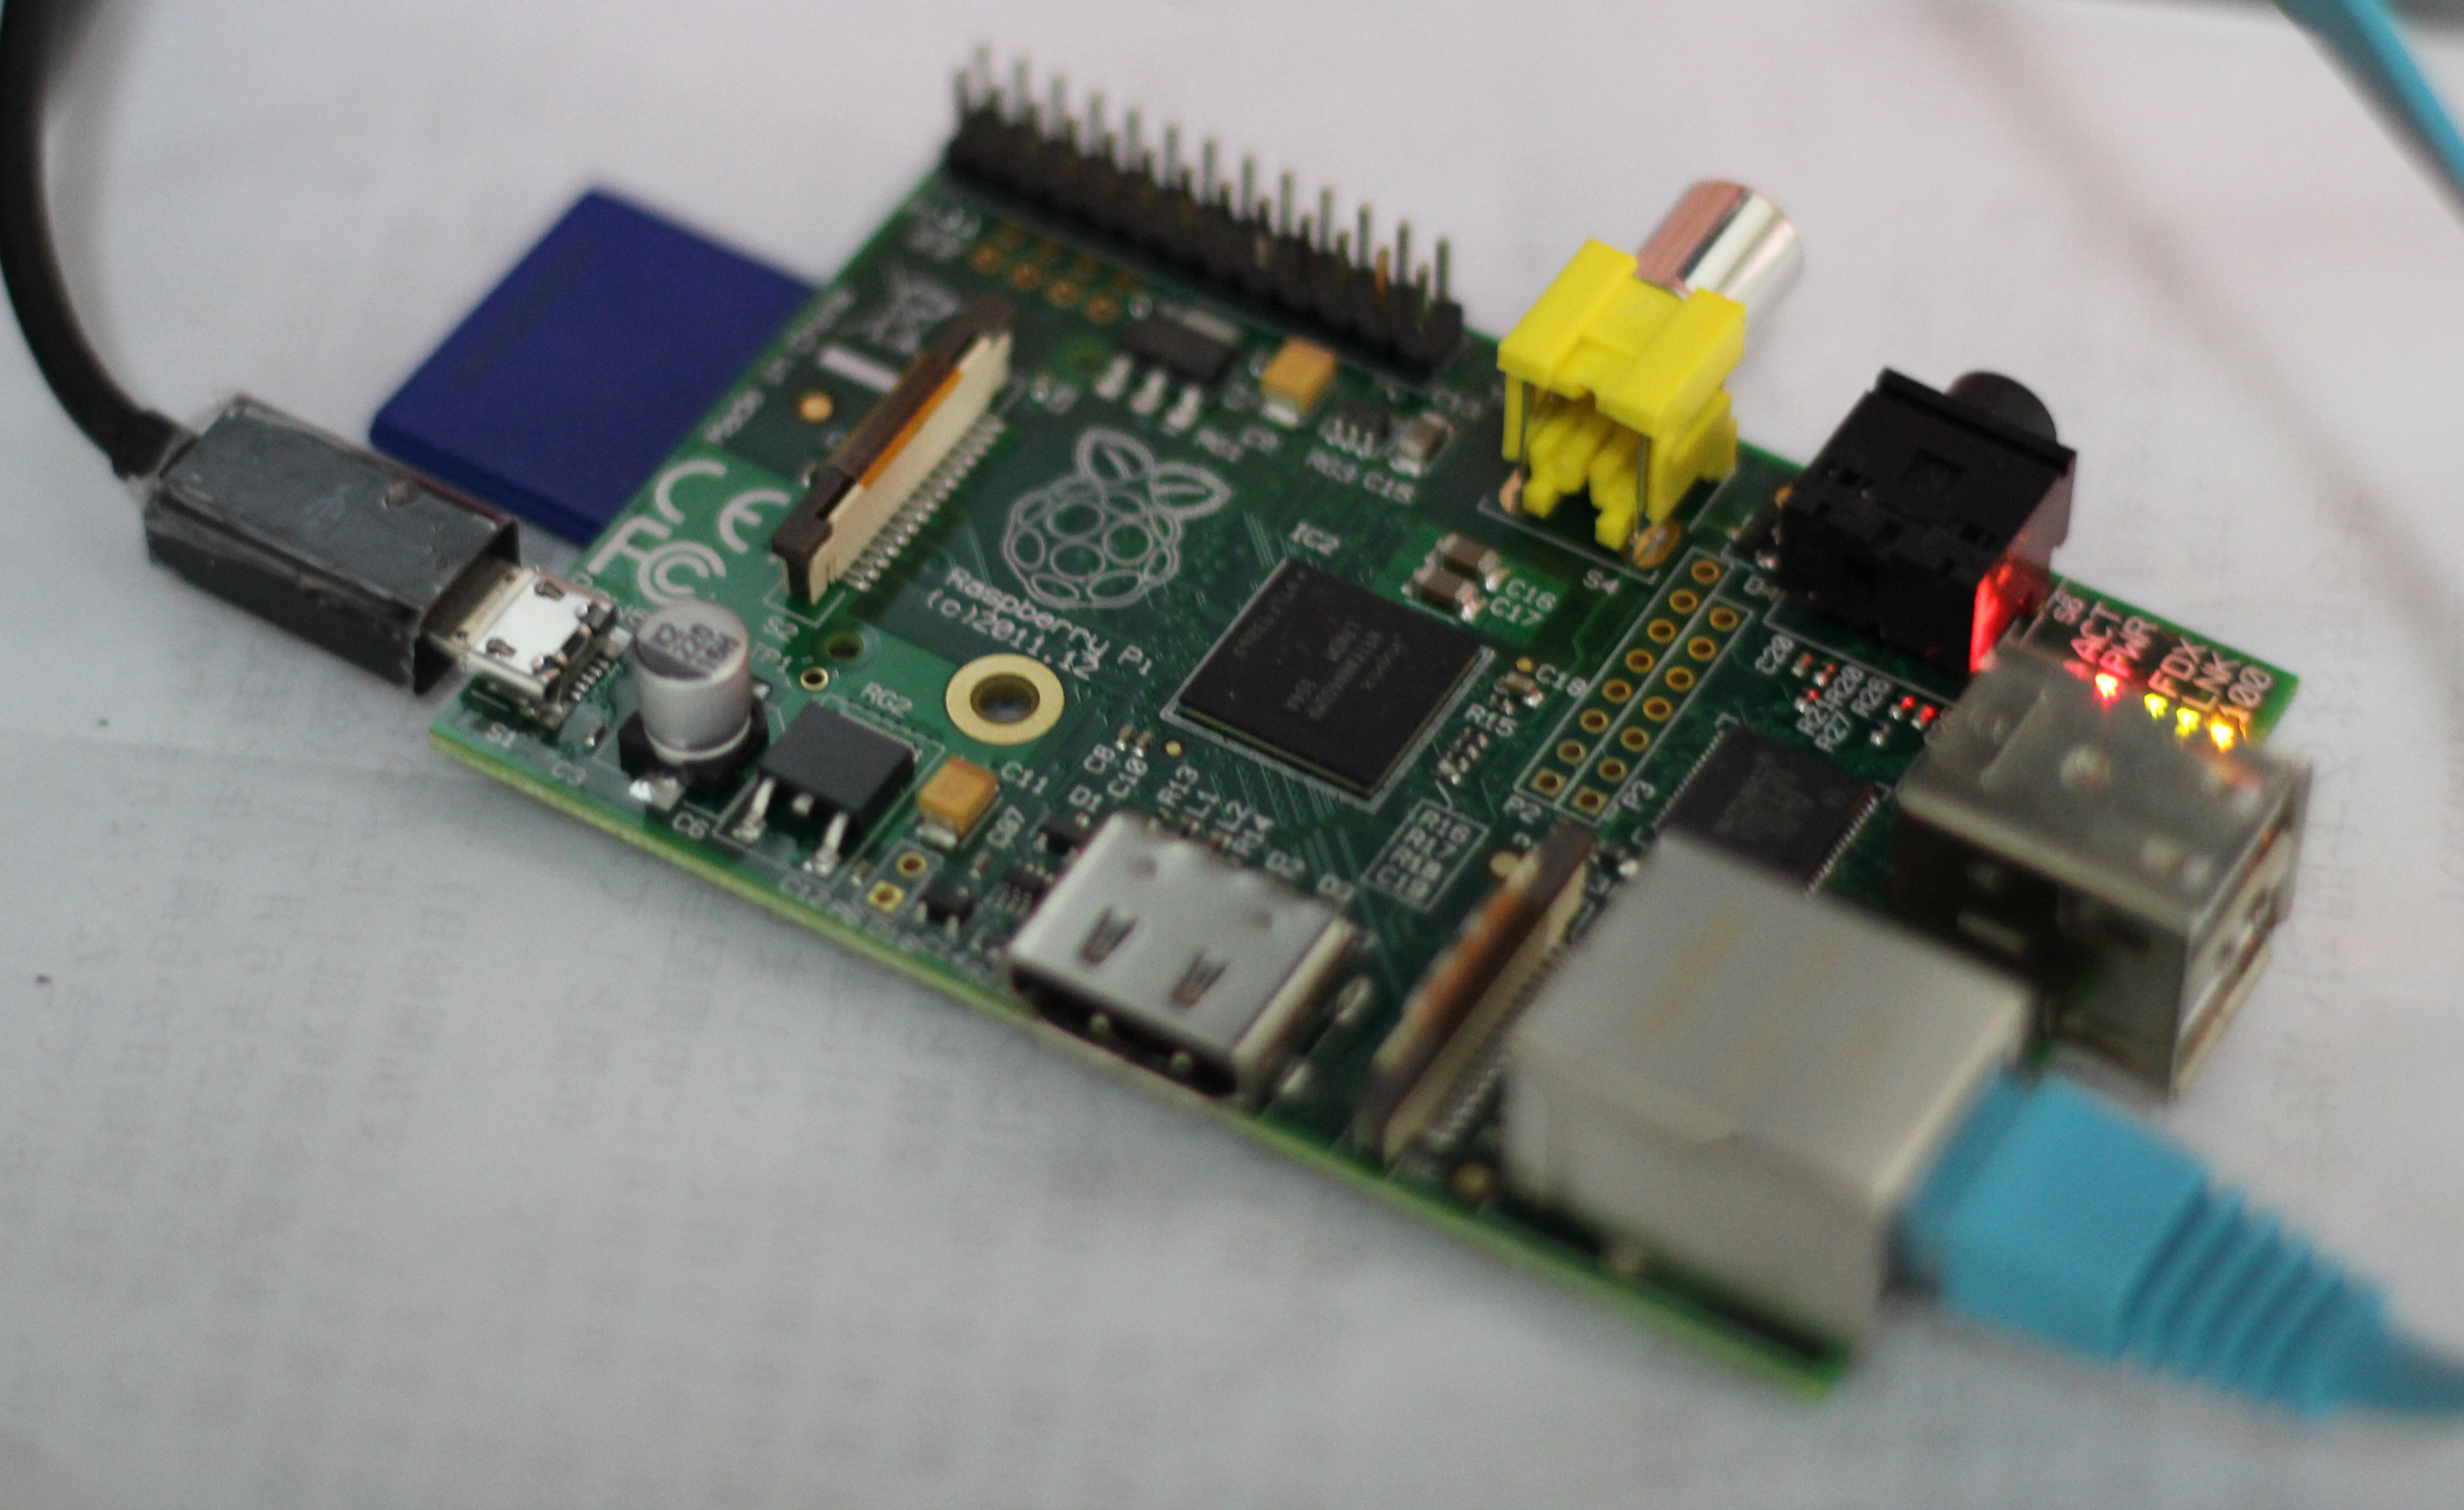
\includegraphics[width=1\hsize]{image201307/raspberrypi.jpg}
\end{frame}

\begin{frame}{raspbian}
 \begin{itemize}
  \item armel: armv4
  \item raspbian: armv6 (VFP2)
  \item armhf: armv7 (NEON)
 \end{itemize}
\end{frame}

\begin{frame}{raspbian$B$N%$%s%9%H!<%k(B}
\begin{itemize}
 \item SD-card $B$K%$%a!<%8$r=q$-9~$s$G$=$l$+$i5/F0$9$k(B
\end{itemize}
\end{frame}

\begin{frame}{$B%5%V%^%7%s$r;H$&;~$NJXMx5;(B}
\begin{itemize}
 \item mosh: ssh $BD%$j$C$Q$J$7$J46$8$K$G$-$F!"%N!<%H%Q%=%3%s%5%9%Z%s%I$7$F$b%j%8%e!<%`(B
       $B$7$?$i$^$?7R$2$i$l$k!#(B
 \item avahi-daemon: DHCP$B$N4D6-$GLLE]$J$3$H$7$J$/$F$b(B
       $B%[%9%HL>;XDj$G%"%/%;%9$G$-$k$h$&$K$J$k!#(Braspberrypi.local 
 \item sshfs: ssh $B$G$D$J$,$k%[%9%H$N%G%#%l%/%H%j$r!!(Bsshfs$B$r;H$C$FF)2aE*(B
       $B$K%^%&%s%H$G$-$k!#(BNFS$B$G%f!<%6(BID$B$rD4@0$7$?$j(BSMB$B$N@_Dj$r4hD%$C$F$7(B
       $B$?$j$7$F$$$?$N$O2a5n$N$3$H$K!#(B
\end{itemize}
\end{frame}


\begin{frame}[containsverbatim]{$B>.5;!'(Bsshfs}
\begin{commandline}
 sshfs corei7.local:path/to/work ./mnt/
\end{commandline}
\end{frame}

\begin{frame}{raspbian$B$N%;%s%5!<(B}
\begin{itemize}
 \item CPU$B29EY%;%s%5!<$r;H$C$F$_$?(B
\end{itemize}
  \includegraphics[width=0.8\hsize]{image201307/temperature.eps}
\end{frame}

\begin{frame}[containsverbatim]{sqlite + R}
$B;~7ONs%G!<%?$r(B sqlite $B$GJ]B8(B
\begin{commandline}
create table temperature(
  timestamp TEXT default current_timestamp,
  temperature INTEGER);
\end{commandline}

$BDj4|E*$K%7%'%k%9%/%j%W%H$G29EY$r=q$-9~$_(B
\begin{commandline}
while sleep 5m; do
    temp=$(cat /sys/class/thermal/thermal_zone0/temp)
    echo "insert into temperature(temperature) " \
 "values($temp);" | \
	sqlite3 sensor.db 
done 
\end{commandline}
\end{frame}

\begin{frame}[containsverbatim]{R $B$G%0%i%U:n@.(B}
$B%?%$%`%>!<%s(BUTC$B$N(BPOSIXct $B7A<0$NJ8;zNs$H$7$F2r<a$5$l$k$N$G$=$l$G=hM}$7$F(B
 $B%0%i%U:n@.(B

\begin{commandline}
library("RSQLite")
drv <- dbDriver("SQLite", max.con=1)
conn <- dbConnect(drv, dbname='sensor.db')
r <- dbGetQuery(conn, 'SELECT * from temperature')
r$posix <- as.POSIXct(r$timestamp, tz='UTC')
plot((temperature / 1000) ~ posix, r,
     xlab='timestamp',
     ylab='temperature C',
     ylim=c(40,60), type='l')
\end{commandline}
\end{frame}

\begin{frame}{$BKM$N(Braspberry pi$B$N:#8e(B}
$BB?J,$3$s$J$3$H$7$^$9!#(B
\begin{itemize}
 \item 1000$B1_$/$i$$$G<j$KF~$k(B WebCam$B$D$1$F4F;k%7%9%F%`(B
 \item $B29EY7W$D$1$F29EYB,Dj(B
\end{itemize}
\end{frame}

\section{$B:#8e$N%$%Y%s%H(B}
\emtext{$B:#8e$N%$%Y%s%H(B}
\begin{frame}{$B:#8e$N%$%Y%s%H(B}
\begin{itemize}
 \item 2013$BG/(B8$B7n(B Debian$BJY6/2q(B
\end{itemize}
\end{frame}

\section{$B:#F|$N1c2q>l=j(B}
\emtext{$B:#F|$N1c2q>l=j(B}
\begin{frame}{$B:#F|$N1c2q>l=j(B}
$BL$Dj(B
\end{frame}

\end{document}

;;; Local Variables: ***
;;; outline-regexp: "\\([ 	]*\\\\\\(documentstyle\\|documentclass\\|emtext\\|section\\|begin{frame}\\)\\*?[ 	]*[[{]\\|[]+\\)" ***
;;; End: ***
